The algorithm proposed by Harms et. al. is well designed but is not capable of finding similar user sequences.
When there is more than one possible interaction to achieve a goal, the method of Harms et. al. will create two different sequences for that interaction,
or worse, will not detect the interaction as a meaningful one at all. For this reason, we propose an algorithm that is able to detect similar subsequences.
The basic steps of the algorithm do not differ a lot from Harms et. al. one. In fact, some preprocessing steps and the sequence detection have been altered.
Algorithm \ref{alg:tasktreeoverview} shows the main building blocks and will function as a list and order of contents of this chapter.
\section{Task Tree Generation}

\begin{algorithm}[h]
\floatname{algorithm}{Algorithm}
\begin{algorithmic}
	\Procedure{GenerateTaskTree}{UserSessions}
	\State Generate Substitution Matrix (UniqueTasks)
	\While{Replaced Tasks}
	\State Detect Iterations (UserSessions)
	\State Optional: Substitution Matrix Update
	\State Detect Sequences (UserSessions,SubstitutionMatrix)
	\EndWhile
	\EndProcedure
\end{algorithmic}
\caption{Overview over the task tree generation}
\label{alg:tasktreeoverview}
\end{algorithm}

\section{Task Distance Substitution Matrix}
The harmonization process performed by Harms et al. is also applied to the user sessions in this approach.
A useful side product of the harmonization is the set of unique tasks.
This set is needed for this step of the algorithm, the generation of the substitution matrix.

In section \ref{sec:foundationsubstitutionmatrix} we introduced substitution matrixes in general and what they are used for.
For the use case of detecting tasks we need to generate one substitution matrix that represents how similar tasks are.
The score of two tasks in the \textit{task distance substitution matrix} is defined as follows:
\begin{definition}
	\item Let a and b be two tasks.
	\item Let S(a,b) = S(b,a) be the score for substituting task a with task b. The higher the value of S is, the more similar are the tasks a and b and vice versa.
\end{definition}

To calculate the score, three cases have to be considered:
\begin{itemize}
	\item Similarity of two event-tasks
	\item Similarity of an event-task and a non-event-task
	\item Similarity of two non-event-tasks
\end{itemize}

\subsection{Event-Task To Event-Task Similarity}
The first idea was to calculate the score of the matrix based on the distance between the absolute coordinates of the event-tasks.
There are a few problems with this approach: First, not all event-tasks may have absolute coordinates.
The second problem with this method is that in graphical user interfaces events may still be very similar, even if they have a large absolute distance.
An example for such a case would be a web formular with many fields to fill out.
TODO: Maybe Screenshot here?
Those fields take space which would result in large distances between them although the event-tasks all belong to a single formular.
The solution to this problems is to make use of a grouping of elements the designer of the GUI already did: The GUI-Model (see section \ref{sec:foundationguiandguimodel}).
Elements of a GUI that belong to one semantic task can usually be found in some kind of container that groups those elements together.
Therefore, the basis for our distance calculation is the distance in the GUI-Model, as defined in \ref{def:guimodeldistanceee}.

\begin{definition}
	\item Let a and b be event-tasks
\begin{equation*}d(a,b) = d(b,a) = \text{the distance in the GUI model of the targets of event-tasks a and b.}
\end{equation*}
\label{def:guimodeldistanceee}
\end{definition}

Since the GUI model is a tree, the distance of two targets in a GUI can easily be calculated by finding the common ancestor of the targets and summing up the number of nodes from both the events to this ancestor, including the ancestor.
\begin{figure}
\begin{center}
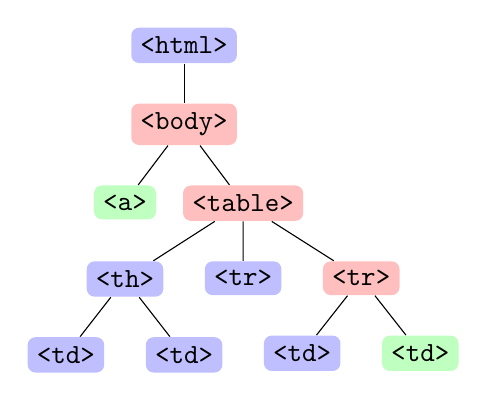
\begin{tikzpicture}[
    fact/.style={rectangle, draw=none, rounded corners=1mm,
        text centered, anchor=north, text=black, fill=blue!25},
    redcolor/.style={rectangle, draw=none, rounded corners=1mm,
        text centered, anchor=north, text=black, fill=red!25},
    greencolor/.style={rectangle, draw=none, rounded corners=1mm,
        text centered, anchor=north, text=black, fill=green!25},
    level distance=0.5cm, growth parent anchor=south]

\node (Fact01) [fact] {\texttt{<html>}} [-]
    child{
        node (kolor4) [redcolor] {\texttt{<body>}}
        child{
            node (color1) [greencolor] {\texttt{<a>}}
        }
        child{
            node (Fact04) [redcolor] {\texttt{<table>}}
            child{
                node (Fact05) [fact] {\texttt{<th>}}
                child{
                    node (fact5) [fact] {\texttt{<td>}}
                }
                child{
                    node (Fact07) [fact] {\texttt{<td>}}
                }
            }
	    child{
                node (Fact05) [fact] {\texttt{<tr>}}
	    }
            child{
                node (color3) [redcolor] {\texttt{<tr>}}
                child{
                    node (Fact10) [fact] {\texttt{<td>}}
                }
                child{
                    node (color2) [greencolor] {\texttt{<td>}}
                }
            }
        }
    }
;

\end{tikzpicture}
\end{center}
\caption{A HTML GUI model with two nodes (green) the distance will be calculated for.  The number of red nodes is the distance between the green nodes. The common anchestor is the \texttt{<body>} element.}
\label{fig:guimodeldistance}

\end{figure}
Figure \ref{fig:guimodeldistance} shows a GUI model with two elements and their common ancestor.


\subsection{Event-Task To Non-Event-Task Similarity}
It takes a bit more effort to calculate the substitution score if one task is a non-event-task.
The reason is that the non-event tasks do not represent a simple event anymore.
Therefore, they do not possess a target in the GUI.
A possible solution is to recursively visit every child of the non-event-task, gather all event tasks and then calculate the mean distance from each of those tasks to the event-task the distance shall be calculated to.
Formally, definition \ref{def:guimodeldistanceee} has to be modified so that it covers non-events as well:

\begin{definition}
%	\item Let a and b be events-tasks, then:
%\begin{equation*}d(a,b) = d(b,a) = \text{be the distance in the GUI model of the targets of event-tasks a and b.}
%\end{equation*}
	\item Let c be a non-event-task.
	\item Let E be the set containing all event-tasks that can be recursively found in c.
	\item With definition \ref{def:guimodeldistanceee} it is possible to define d as
\begin{equation*}
	d(a,c) = d(c,a) = \frac{\sum_{\forall x \in E} d(a,x)}{|E|}
\end{equation*}
\label{def:guimodeldistanceene}
\end{definition}

\subsection{Non-Event To Non-Event Similarity}
With Definition \ref{def:guimodeldistanceene} it is simple to compute the distance for two tasks since all that is to do now is to repeat the procedure of finding all event-task children of one task, calculate the distances to the other task and use the mean distances as the total distance.
The definition of d can be extended so it accepts two non-event-tasks:

\begin{definition}
	\item Let c and d be non-event-tasks.
	\item Let E be the set containing all event-tasks that can be recursively found in c.
	%\item Let F be the set containing all event-tasks that can be recursively found in d.
	\item With definition \ref{def:guimodeldistanceene} it is possible to define d as
	\begin{equation*}
		d(c,d) = d(d,c) = \frac{\sum_{\forall x \in E} d(x,d)}{|E|}
	\end{equation*}
\label{def:guimodeldistancenene}
\end{definition}
\subsection{Score}
Now that we defined the distance for three cases it is possible to compute the score $S$ of two tasks.
To transform a distance into a score we multiply all distance values with $-1$ and add a constant so that some scores are positive and some have a negative value.

\begin{definition}
	\item Let U be the set of unique tasks occurring in the user sessions.
	\item Let k be a constant that defines the maximal score.
	\item For each tupel $i,j \in U$
\begin{equation*}
		 S(i,j) = -1*d(i,j)+k
	\label{eq:subscore}
\end{equation*}
\label{def:scorewithmaximalscore}
\end{definition}
The $k$ constant should be chosen dependent on the underlying GUI model.
A large k may be chosen for very deeply, nested GUI models whereas for flat GUI models a smaller $k$ seems better.
At last this parameter has to be evaluated and carefully adjusted to the given input data.

The maximal score is reached if the distance between two elements is zero. This happens if we compare two equal elements.
A problem can occur when the score of a non-event-task to an event task is equal to maximal score.
This happens if a non-event-task has just one event-task as child and the distance of this child to the same event-task is calculated.
Since it is preferred that the score of two equal event-tasks is always larger than the score of this event-task with a non-event-task we add the penalty term $L$ to the score equation.

\begin{definition}
	\item Let E be the set of all event-tasks.
	\item Let N be the set of all non-event-tasks.
\begin{eqnarray*}
	L(i,j) &=&
	\begin{cases}
		0 & \text{if } i,j \in E \\
		\text{constant} & \text{if } i \in N \lor  j \in N\\
	\end{cases} \\
	S(i,j) &=& -1*d(i,j)+k-L
	\label{eq:subscore_adjusted}
\end{eqnarray*}
\label{def:scoreadjusted}
\end{definition}


\section{Iteration Detection And Substitution Matrix Update}
The iteration detection from Harms is also suitable for our algorithm and was not altered in any way. It reliably detects iterations and replaces them in the user sessions.
Before the sequence detection can come into play, the substitution matrix should be updated since there were new iteration tasks created during iteration detection. Those new tasks are stored in a set that contains all newly created tasks.
The update process differs just a little from the generation process with the only difference beeing that just the distances between the newly created tasks to the current set of unique tasks is as well as the distances between the newly created tasks are computed.
After the matrix has been updated, the newly created tasks are merged with the set of unique tasks and then emptied.

The update process is a very expensive procedure. An alternative to this is to set each score between an event-task to a non-event-task and therefore all scores between non-event-tasks to zero.
Both variants are evaluated in chapter \ref{chap:casestudy}.

\section{Sequence Detection}
As we figured out at the beginning of this chapter the sequence detection is the part of the algorithm that varies the most from Harms approach.
It is itself separated in four steps:
\begin{enumerate}
	\item The search for significant patterns
	\item The match retrival
	\item The task generation
	\item The sequence replacement
\end{enumerate}

\subsection{Search For Significant Patterns}
The search for significant patterns is done with an alignment method we introduced in section \ref{sec:alignments}.
The bioinformatical problem of comparing and aligning DNA/RNA/Amino acid sequences is closely related to finding more or less equal subsequences in the user sessions.
The conserved regions of biological sequences comply with those interactions that most of the users performed similarly.
We can conclude that those interactions are meaningful in the sense of fulfilling one desired task.
The goal of the alignment algorithm is now to detect the conserved regions and extract a model of the average user behaviour.
Since alignment algorithms also find approximate and not only exact similarities, this step of the sequence detection is the main difference to Harms method.

The first step of the search for significant patterns is to align every user session with any other user session with the Smith-Waterman algorithm for repeated matches.
For the rest of this section the user session will be represented by a sequence of numbers. Each number in a sequence corresponds with the unique id of the task at this position in the user sessions.
We now describe the algignment algorithm in detail.

\subsubsection{Smith Waterman Algorithm for Repeated Matches}
The Smith-Waterman algorithm for repeated matches\cite{durbin1998} is a modified version of the original Smith-Waterman algorithm\cite{waterman1981}.
The original Smith-Waterman finds the best local similarity between two sequences.
Since we need all relevant similarities and not just the one with the best score, we define a threshold score $T$.
\begin{definition}
	Let T be the threshold score for subalignments.
	\label{def:treshold}
\end{definition}
Once a local subalignment reaches T it is considered as relevant.

We recall from the section \ref{sec:alignments} that alignment algorithms try to find the best possible score between two sequences using the underlying scoring model of substitution and gap scores.
The most na\"ive approach is to test possible combinations both sequences could be aligned. As usual, this approach is not very feasible because there are
\begin{equation*}
	\binom{2n}{n} = \frac{(2n)!}{(n!)^2} \simeq \frac{2^{2n}}{\sqrt{\pi n}}
\end{equation*}
possible global alignments of two sequences\cite{durbin1998}.
Another way would be to use some kind of heuristic but we are interested in an exact, deterministic method.
A common technique to solve this issue is dynamic programming\cite{bellman1957}.
The main idea of dynamic programming is not to calculate every possible variant but to reuse the best solutions of smaller subproblems.
This method is central to computational sequence analysis\cite{durbin1998}.

\paragraph{Basic Smith-Waterman}
The basic version of the Smith-Waterman algorithm makes use of dynamic programming by defining the dynamic programming matrix $F$ where each cell of the matrix stores the best score for aligning the elements up to the position the cell represents.
For example the cell $(2|2)$ stores the score for the best alignment of first two elements of each sequence.
Each cell is computed by getting the best score out of four choices. Prior to enlisting those, we need the following definitions:

\begin{definition}
	\item Let x,y be two sequences.
	\item Let F be a matrix with F(i,j) being the best score of aligning $x_1\dots x_i$ with $y_1\dots y_j$.
\end{definition}
Then we can compute F by repeatedly applying the following equation:
\begin{equation}
F(i,j) = max \left\{ \begin{array}{lr}0,&\\F(i-1,j-1)+S(x_i,y_j),&Substitution\\F(i-1,j)-g,&Gap\\F(i,j-1)-g.&Gap\\\end{array} \right.
\end{equation}
Figure \ref{fig:basicalignmentoperations} illustrates this formula.
The diagonal choice means we align one element from each sequence with each other.
Therefore, we have to look up the similarity of both elements in the substitution matrix.
When the score from the upper cell minus the gap penalty is bigger than the diagonal choice a gap will appear at this position in sequence y.
This is the same for when the option from the left cell is taken, just that the gap will be inserted in sequence x.
The option 0 in the equation is to prevent alignment scores to become negative.
If a match cannot be extended with its score being a positive value, it is better to start a new one later.
As we can see, it is possible to fill the whole matrix by once the trivial scores, the first row and the first column, have been initialized.

\begin{figure}
	\centering
	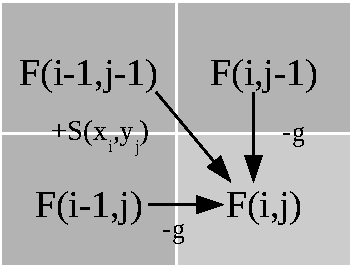
\includegraphics{img/basic_cell_fill.pdf}
	\caption{Illustration of the three operations deletion, insertion and substitution in a dynamic programming matrix.}
	\label{fig:basicalignmentoperations}
\end{figure}

\paragraph{Repeated matches}
In the improved version of the algorithm a cell in $F$ has a slight different meaning and its computation is a bit more complex.
The first difference is that this algorithm is asymmetric in the sense of aligning sequence x to sequence y produces a different outcome than aligning sequence y to sequence x.
Hence, we define y as the pattern we want to search and x as the sequence in which we search all subsequences of y repeatedly.
This results in a final alignment where x has matched and unmatched regions.

The algorithm itself is partitioned into three parts:

\begin{itemize}
	\item Initialization
	\item Recursion
	\item Traceback
\end{itemize}

\subparagraph{Intialization}
	The initialization step is simple: \\
	Let m be the length of y

	\begin{equation*}
		F(0,j) = 0 \text{ for } j=0\dotsc m
	\end{equation*}
	This differs from the Smith-Waterman algorithm described by Durbin et al.\cite{durbin1998} who just initialize F(0,0) and do not fill the first column. There is no need to initialize the first row because a subalignment will never start with a gap. For the sake of an easy implementation it was better to initialize the first row though.

\subparagraph{Recursion}
The recursion formula for filling the matrix also has the three options for insertion, deletion and substitution as illustrated in figure \ref{fig:basicalignmentoperations}.
But as we see there are some more options.
For the first row (equation \ref{eq:firstrow}), which does not represent a real alignment of sequences but denotes the sum of completed match scores, we have two options.
The first one is to take the value from the last column so we always keep track of the total score.
This leads to the fact that the value in this line will always stay the same or increase, but never decrease.
The second choice is taken when a match reaches its maximum and has a minimum score of T.
This is the consequence of an ending match meaning this choice is just taken when we calculate the cell for an unmatched region.
To summarize the equation for the first row we can say the algorithm choses the maximum value of the last column minus T or adopts the value of the preceding cell in the first row, depending which one was larger.

Equation \ref{eq:otherrows} for the fields aside of the first row is amended by the posibility to begin its alignment score with the value standing in the first row of its own column.
Durbin et al. do not mention the fact that this makes it easier for subalignments of long sequences to reach the threshold score once a few matches have been found before.
This issue has not been investigated in this work.
The total score of the whole alignment is stored in F(i+1,0). This cell lies in an unmatched region of x and contains the sum of all completed match scores.


\begin{equation}
F(i,0) = max \left\{ \begin{array}{lr}F(i-1,0),&\\F(i-1,j)-T,& j=1,\dots,m\end{array}\right.
\label{eq:firstrow}
\end{equation}
\begin{equation}
F(i,j) = max \left\{ \begin{array}{lr}F(i,0),\\F(i-1,j-1)+S(x_i,y_i),\\F(i-1,j)-g,\\F(i,j-1)-g.\end{array}\right.
\label{eq:otherrows}
\end{equation}

\subparagraph{Traceback}
A very important point in dynamic programming algorithms is that we not just calculate and store the maximum score for each subproblem but additionally have to store which choice of the formula produced the highest value.
This makes it possible to go back from the total best score to the start and find the actual alignment of the whole sequences.
This process is called traceback.
The procedure is to go back the path that led to the final score (here in F(i+1,0)).
After going back, again take the path that led to the previous cell. Repeat this procedure until F(0,0) is reached.
Figure \ref{fig:durbindpmatrixtraceback} shows a completely filled dynamic programmic matrix and the traceback path.

\begin{figure}
\centering
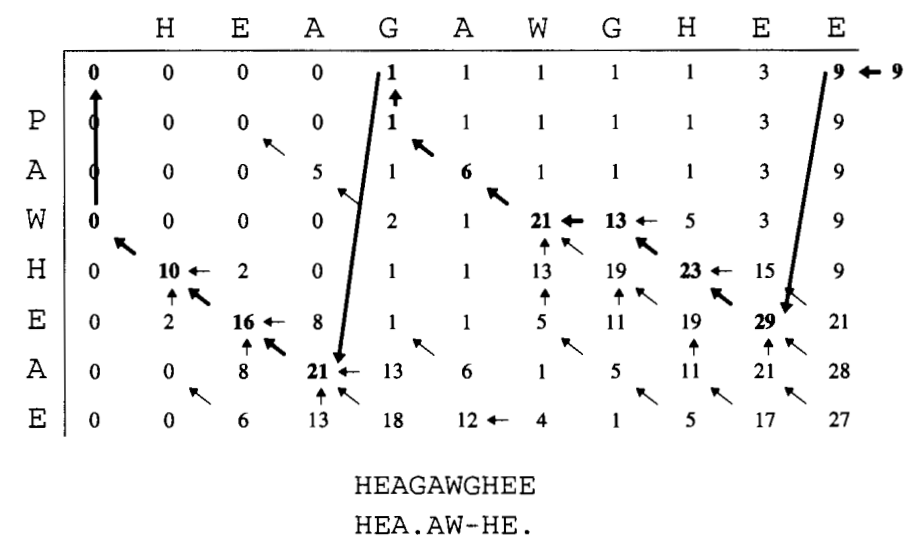
\includegraphics[scale=0.4]{chapters/approach/smithwatermanrepeated.png}
\caption{Figure from Durbin et al.\cite{durbin1998}. The repeat dynamic programming matrix for two example sequences, for T = 20. Below the optimal alignment, with total score \mbox{$9 = 29-20$}. There are two separate match regions, with scores 1 and 8. Dots are used to indicate unmatched regions of x. The arrows show the traceback process, going back from the total score to the start.}
\label{fig:durbindpmatrixtraceback}
\end{figure}

\subsection{Match retrival}
To find similar user behaviour we are only interested in the matches that reached the threshold score.
After aligning every user session with each other we extract all matches from those alignments.
We consider every subset of the alignment that is not an unmatched region as a match.
Therefore, a match consists of two sequences of numbers and can contain gaps.
We encode a gap with the value -1.
Figure \ref{fig:matchexample} shows an example of a match, containing one gap in the first sequence, two exact tasks and one substitution.

\begin{figure}[h]
	\centering
	\begin{tabular}{cccc}
		9 & 16 & -1 & 6 \\
		9 & 15 & 17 & 6
	\end{tabular}
	\caption{Example for a retrieved match. Each of the two subsequences of the sequences the match was generated from is printed in a row.}
	\label{fig:matchexample}
\end{figure}
Each of those matches is searched in all user sessions.
For this, each position in the user sessions is checked if the match in question fits at this position.
Before we can do this, we have to explain what it means that a match is found since we have to take into account how a match will be transformed into a task later.
When a match is found we store the id of the user session it occured in as well as its position in the user session.
There are some rules that have to be fulfilled to consider a match as found:

	\begin{rules}
		\item If both elements of a position in a match are equal, this element has to be found at this position of the subsequence in which we search.
	\end{rules}
	\begin{figure}[h]
		\centering
			\begin{tabular}{cc}
				 16 & 4\\
				 16 & 4\\
			\end{tabular}
		\caption{Example for rule 1. Will only match a user session subsequence 16 4.}
		\label{fig:rule1}
	\end{figure}


	\begin{rules}
		\item If one element in a match is a gap (-1), the other element of this position is optional at this position.
	\end{rules}
	\begin{figure}[h]
		\centering
			\begin{tabular}{ccc}
				16 & -1 &6\\
				16 &  4 & 6\\
			\end{tabular}
			\caption{Example for rule 2. Will match user session subsequences 16 4 6 and 16 6.}
		\label{fig:rule2}
	\end{figure}

	\begin{rules}
	\item If both elements are not equal and the next position contains two equal elements (a) or a gap (b), either of the unequal elements can occur at this position.
	\end{rules}
	\begin{figure}[h]
		\centering
		\begin{subfigure}[b]{0.49\textwidth}
		\centering
			\begin{tabular}{cc}
				 14 & 4\\
				 16 & 4\\
			\end{tabular}
			\caption{Example for rule 3 (a). Will match 16 4 and 14 4.}
			\label{fig:rule3}
		\end{subfigure}
		\begin{subfigure}[b]{0.49\textwidth}
		\centering
			\begin{tabular}{ccc}
		\centering
				14 & -1 & 6\\
				16 & 4  & 6 \\
			\end{tabular}
			\caption{Example for rule 3 (b). Will match 16 4 6, 14 4 6, 14 6 and 16 6. }
		\end{subfigure}
		\caption{Examples for rule 3 (a) and (b).}
		\label{fig:rule3}
	\end{figure}
	\begin{rules}
	\item If both elements are not equal and the elements of the next positions are not equal as well:
		\begin{enumerate}
			\item Group all elements of one sequence together as long as the next positions still have unequal elements.
			\item A match is found if the user session matches completely one of those grouped sequences.
		\end{enumerate}
	\end{rules}
	\begin{figure}[h]
	\centering
	\begin{tabular}{ccc}
		 16 & 18 & 14 \\
		 15 & 17 & 16 \\
	\end{tabular}
	\caption{Example for rule 4. Match is found if a subsequence of a user session is 15,17,16 or 16,18,14 but not 15,18,14.}
	\label{fig:rule4}
	\end{figure}

\paragraph{Match Sorting}
Once all matches have been retrieved they have to be sorted to have an order they will be replaced in the sequences. The sorting criteria are the following:
First we sort by the number of occurence in all sequences.
The reason for this is that we want to prefer the most occurring match over all other match properties because it is likely that a task with a high occurence represents
the average user behaviour. If two matches have the same occurrence count, the length of the matches is considered. Longer matches will be replaced first.
The next two sort properties are introduced for a deterministic behaviour of the algorithm.
%The reason why is that we need an explicit order of all matches.
If two matches have the same occurrence count and the length, the sum of the user session ids is considered and after that the sum of the task ids.


\subsection{Task generation}
After sorting the matches, the actual task is created from each match that has a minimum occurence of f.
This parameter is introduced to exclude those matches that just have been performed by a small number of users and therefore are not representative for a general interaction with the software.
\begin{definition}
	\item Let f be the number of occurrences a task must have in all user sessions in order to be replaced.
		\label{def:minoccurrencecount}
\end{definition}
We will now see why we had to search the matches according to the rules enlisted in the previous section. The task generation rules correspond to the search rules.
We start with an empty task of temporal relationship type \textit{sequence}.
This is the root node of the task we will convert the match to.
For this, the procedure is to evaluate each position of the match and apply some rules again.
If both elements in the match are equal, the task with this id is added to the sequence. This is the equivalent to search rule 1.
Search rule 2 transferred to task generation leads to the creation of tasks with temporal relationship type \textit{optional}.
The created optional task has the task that is "aligned" with the gap as its child.
If the algorithm observes a position where search rule 3 is applied, a single selection with two children is created.
Both of the two unequal tasks of this position have this selection as their parent.
The adopted application of search rule 4 creates three new tasks, a selection and two sequences.
The selection is added to the root sequence, both of the sequences are children of the selection.
The sequences themselves contain the subsequent unequal tasks of one row of the match.
Figure \ref{fig:matchexampletaskgeneration} shows a match that is converted into a task. In this match all rules have been applied.

\begin{figure}[h]
	\centering
	\begin{subfigure}[c]{0.44\textwidth}
		\centering
	\begin{tabular}{cccccc}
		9 & 16 & -1 & 6 & 4& 5\\
		9 & 15 & 17 & 5 & 3& 5\\
	\end{tabular}
	\end{subfigure}
	\begin{subfigure}[c]{0.1\textwidth}
		\centering

		\Large{$\Rightarrow$}
	\end{subfigure}
	\begin{subfigure}[c]{0.44\textwidth}
		\tikzstyle{every node}=[rectangle, draw=none, rounded corners=1mm,
		        text centered, anchor=west, text=black, fill=blue!30]

		\begin{tikzpicture}[%
		  grow via three points={one child at (0.5,-0.7) and
		  two children at (0.5,-0.7) and (0.5,-1.4)},
		  edge from parent path={(\tikzparentnode.south) |- (\tikzchildnode.west)}]
		  \node {Sequence}
		  	child { node {9} }
		  	child { node {Selection}
		        	child { node {16}}
		        	child { node {15}}
		        }
		 	child [missing] {}
		 	child [missing] {}
		        child { node {Optional}
		        	child { node {17}}
		        }
		 	child [missing] {}
		        child { node {Selection}
		        	child { node {Sequence}
		        		child{node {6}}
		        		child{node {4}}
		        	}
		 		child [missing] {}
		 		child [missing] {}
		        	child{ node {Sequence}
		        		child{node {5}}
		        		child{node {3}}
		        	}
		        }
		 	child [missing] {}
		 	child [missing] {}
		       child { node {5}};

		    \end{tikzpicture}
	\end{subfigure}
	\caption{Example for task generation. The match on the left is converted into the task on the right.}
	\label{fig:matchexampletaskgeneration}
\end{figure}

\subsection{Replacement}
One last step is required to finish the sequence detection: the replacement of all generated tasks in all the user sessions.
For this we create an instance of the generated sequence and replace each subsequence in the user sessions that fits the model of the instance.
We do not need to search the positions where we can insert the instance since we stored all the occurrences in our first search.
What we have to do is to update the information about the position in all other stored match occurrence data.
For example, if we extract six task instances, match occurrences with a position after this replacement need to substract six from their start and end indices.
If a first replacement overlaps another one, the second one is ignored. Here we can see again that the order of replacement is very important  because it determines which
matches are replaced and which may be ignored.

\subsection{Repetition}
Same as in Harms et al.s approach the steps iteration detection and sequence detection are repeated until a specific condition is reached.
Harms et al. repeat until no further replacements can be made.
We propose to stop the repetition before.
Possible conditions could be that the algorithms stops once it finds less matches than a specific percentage of the number of matches that have been found in the first iteration of the algorithm.
Another possibility would be to have a fixed number of iterations.
We will evaluate those proposals in the case study section.
